\documentclass{article}

% plain R
% chunk and its name
% fig


\usepackage{Sweave}
\begin{document}
\Sconcordance{concordance:paperVersion_0.tex:paperVersion_0.Rnw:%
1 7 1 1 0 18 1 1 3 2 0 1 1 3 0 1 2 2 1 1 2 1 0 1 1 7 0 1 2 1 1 1 2 1 0 %
1 1 7 0 1 2 1 1 1 2 1 0 1 1 1 3 7 0 1 3 2 1 1 2 1 0 1 1 7 0 1 2 2 1 1 2 %
1 0 1 1 7 0 1 2 1 1 1 2 1 0 1 1 1 3 7 0 1 3 2 1 1 2 1 0 1 1 7 0 1 2 2 1 %
1 2 1 0 1 1 7 0 1 2 1 1 1 2 1 0 1 1 1 3 6 0 1 2 2 1 1 2 1 0 1 1 7 0 1 2 %
2 1 1 2 1 0 1 1 7 0 1 2 2 1 1 2 1 0 1 1 1 3 6 0 1 2 2 1 1 2 25 0 1 2 4 %
1 1 2 1 0 1 4 3 0 1 1 7 0 1 2 5 1 1 3 2 0 1 3 1 0 1 1 15 0 1 2 2 1 1 2 %
1 0 1 1 27 0 1 3 2 1 1 2 1 0 1 1 25 0 1 2 5 1}


LOS INDICES DEL MUNDO


Por: Estrella Delcurso


Introducción

Aqui les presento mi investigacion sobre diversos indices sociales en el mundo. Los indices los conseguí de wikipedia, espero que les gusten mucho.


Exploración Univariada

En esta sección exploro cada índice.


\begin{Schunk}
\begin{Sinput}
> # carga de datos
> filename="indexes.csv"
> dataidx=read.csv(filename, stringsAsFactors = T)
\end{Sinput}
\end{Schunk}


Este es el comportamiento de la democracia en el mundo, veamos primero las frecuencias absolutas:
\begin{Schunk}
\begin{Sinput}
> demoTable=table(dataidx$Democracy)
> demoTable
\end{Sinput}
\begin{Soutput}
 1 very bad       2 bad      4 good 5 very good 
         50          40          77          19 
\end{Soutput}
\end{Schunk}

Ahora las frecuencias relativas:
\begin{Schunk}
\begin{Sinput}
> demoTableRel=round(prop.table(demoTable)*100,1)
> demoTableRel
\end{Sinput}
\begin{Soutput}
 1 very bad       2 bad      4 good 5 very good 
       26.9        21.5        41.4        10.2 
\end{Soutput}
\end{Schunk}

Y aquí el plot que representa esta distribución
\begin{Schunk}
\begin{Sinput}
> title='Distribución de la Democracia'
> paleta='red'
> barplot(demoTableRel,main=title,
+         col=paleta,ylim = c(0,100),
+         ylab = "%")
> 
\end{Sinput}
\end{Schunk}
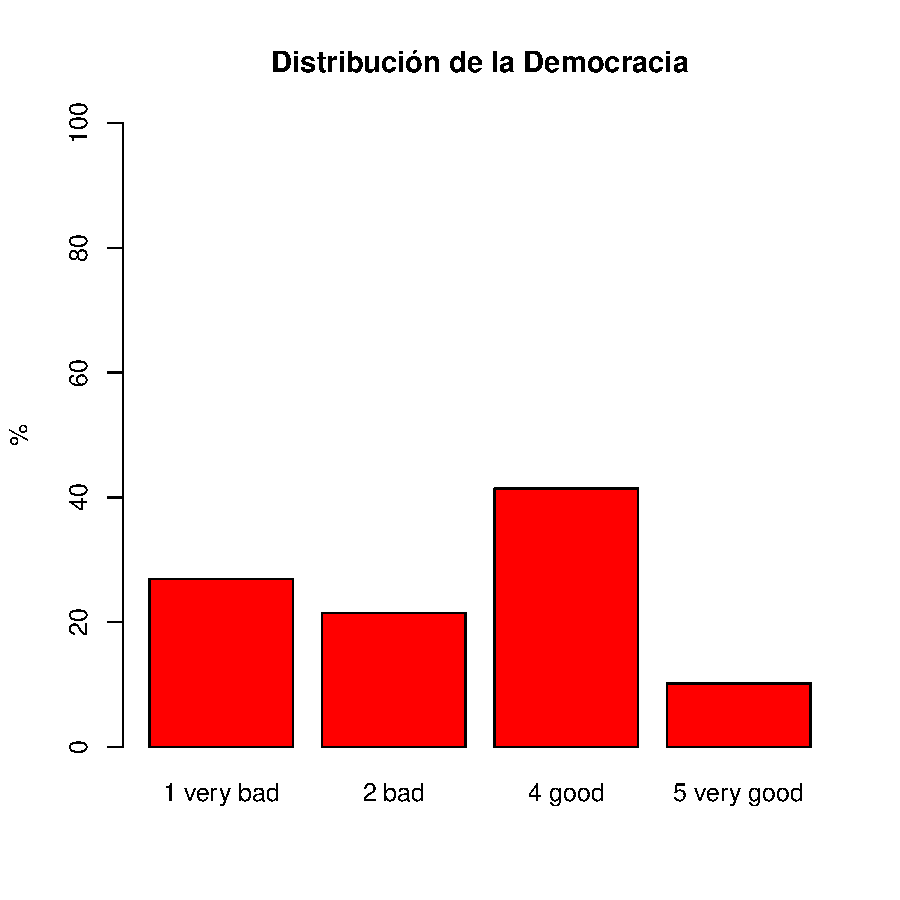
\includegraphics{paperVersion_0-demoTableRelPlot}


La Libertad económica en el mundo en una tabla:
\begin{Schunk}
\begin{Sinput}
> ecoTable=table(dataidx$EconomicFreedom)
> ecoTable
\end{Sinput}
\begin{Soutput}
 1 very bad       2 bad    3 middle      4 good 5 very good 
         18          65          71          26           6 
\end{Soutput}
\end{Schunk}


Ahora las frecuencias relativas:
\begin{Schunk}
\begin{Sinput}
> ecoTableRel=round(prop.table(ecoTable)*100,1)
> ecoTableRel
\end{Sinput}
\begin{Soutput}
 1 very bad       2 bad    3 middle      4 good 5 very good 
        9.7        34.9        38.2        14.0         3.2 
\end{Soutput}
\end{Schunk}

Y aquí el plot que representa esta distribución
\begin{Schunk}
\begin{Sinput}
> title='Distribución de la Libertad Económica'
> paleta='red'
> barplot(ecoTableRel,main=title,
+         col=paleta,ylim = c(0,100),
+         ylab = "%")
> 
\end{Sinput}
\end{Schunk}
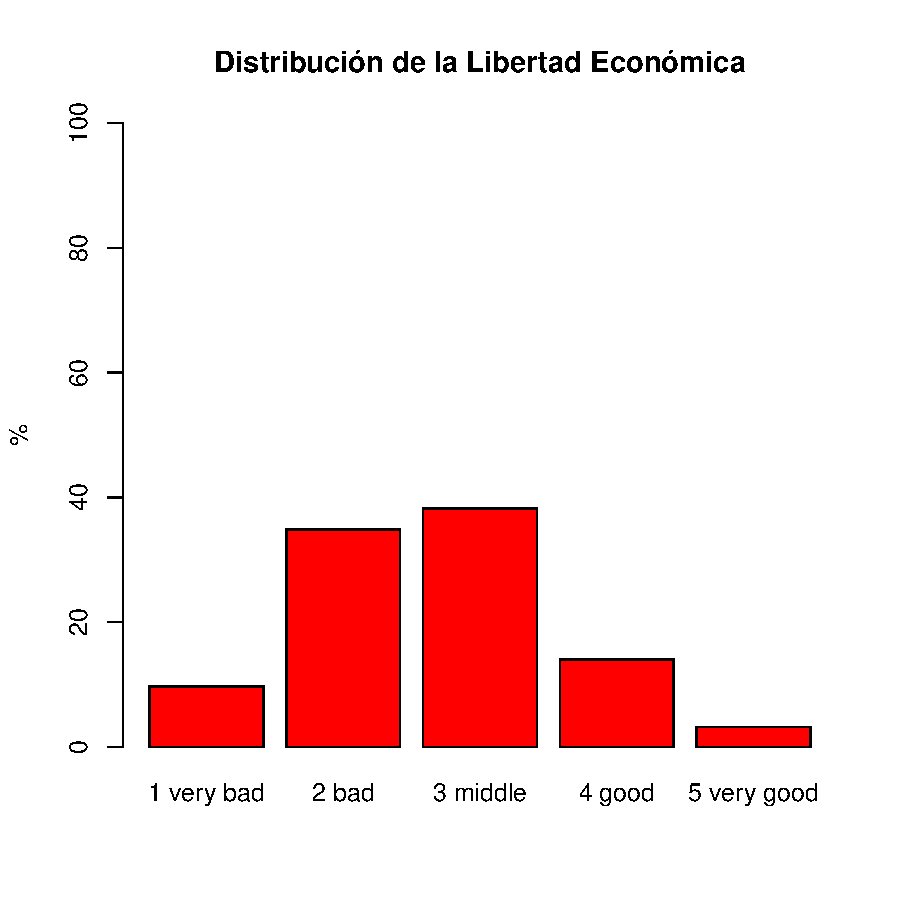
\includegraphics{paperVersion_0-ecoTableRelPlot}


La Libertad general en el mundo en una tabla:
\begin{Schunk}
\begin{Sinput}
> worldTable=table(dataidx$WorldFreedom)
> worldTable
\end{Sinput}
\begin{Soutput}
 1 very bad    3 middle 5 very good 
         46          56          84 
\end{Soutput}
\end{Schunk}


Ahora las frecuencias relativas:
\begin{Schunk}
\begin{Sinput}
> worldTableRel=round(prop.table(worldTable)*100,1)
> worldTableRel
\end{Sinput}
\begin{Soutput}
 1 very bad    3 middle 5 very good 
       24.7        30.1        45.2 
\end{Soutput}
\end{Schunk}

Y aquí el plot que representa esta distribución
\begin{Schunk}
\begin{Sinput}
> title='Distribución de la Libertad en el Mundo'
> paleta='red'
> barplot(worldTableRel,main=title,
+         col=paleta,ylim = c(0,100),
+         ylab = "%")
\end{Sinput}
\end{Schunk}
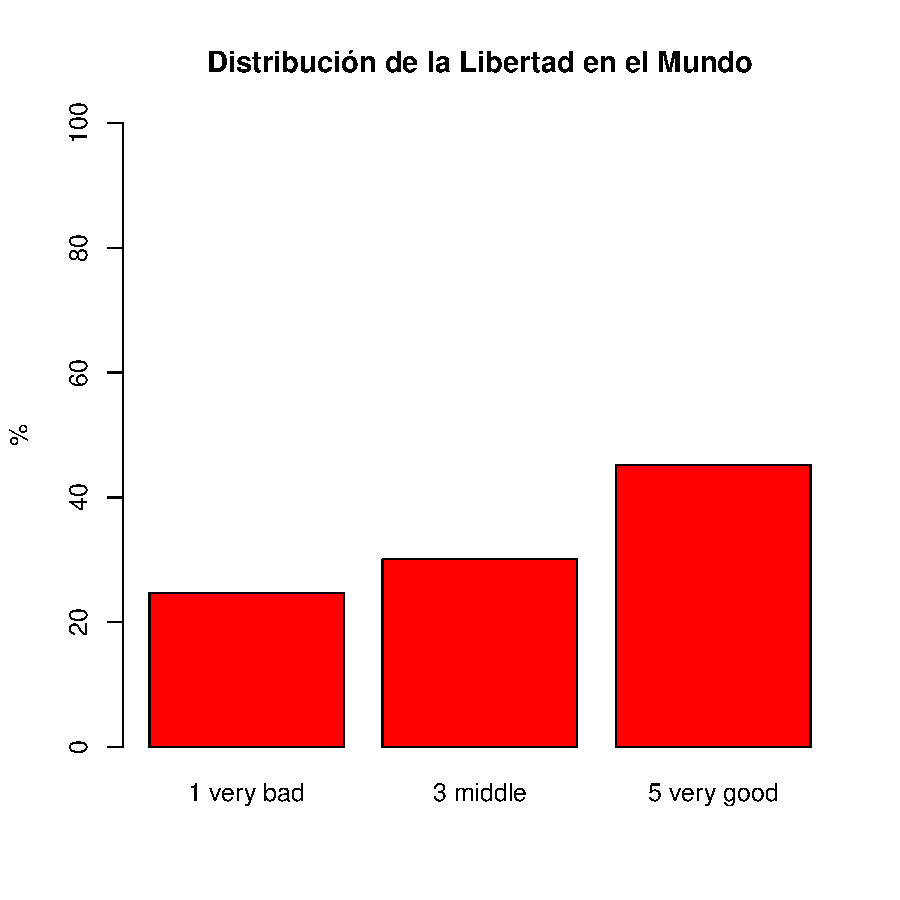
\includegraphics{paperVersion_0-worldTableRelPlot}


La Libertad de prensa en el mundo en una tabla:
\begin{Schunk}
\begin{Sinput}
> pressTable=table(dataidx$PressFreedom)
> pressTable
\end{Sinput}
\begin{Soutput}
 1 very bad       2 bad    3 middle      4 good 5 very good 
         20          44          60          45          17 
\end{Soutput}
\end{Schunk}


Ahora las frecuencias relativas:
\begin{Schunk}
\begin{Sinput}
> pressTableRel=round(prop.table(pressTable)*100,1)
> pressTableRel
\end{Sinput}
\begin{Soutput}
 1 very bad       2 bad    3 middle      4 good 5 very good 
       10.8        23.7        32.3        24.2         9.1 
\end{Soutput}
\end{Schunk}


Y aquí el plot que representa esta distribución
\begin{Schunk}
\begin{Sinput}
> title='Distribución de la Libertad de Prensa'
> paleta='red'
> barplot(pressTableRel,main=title,
+         col=paleta,ylim = c(0,100),
+         ylab = "%")
\end{Sinput}
\end{Schunk}
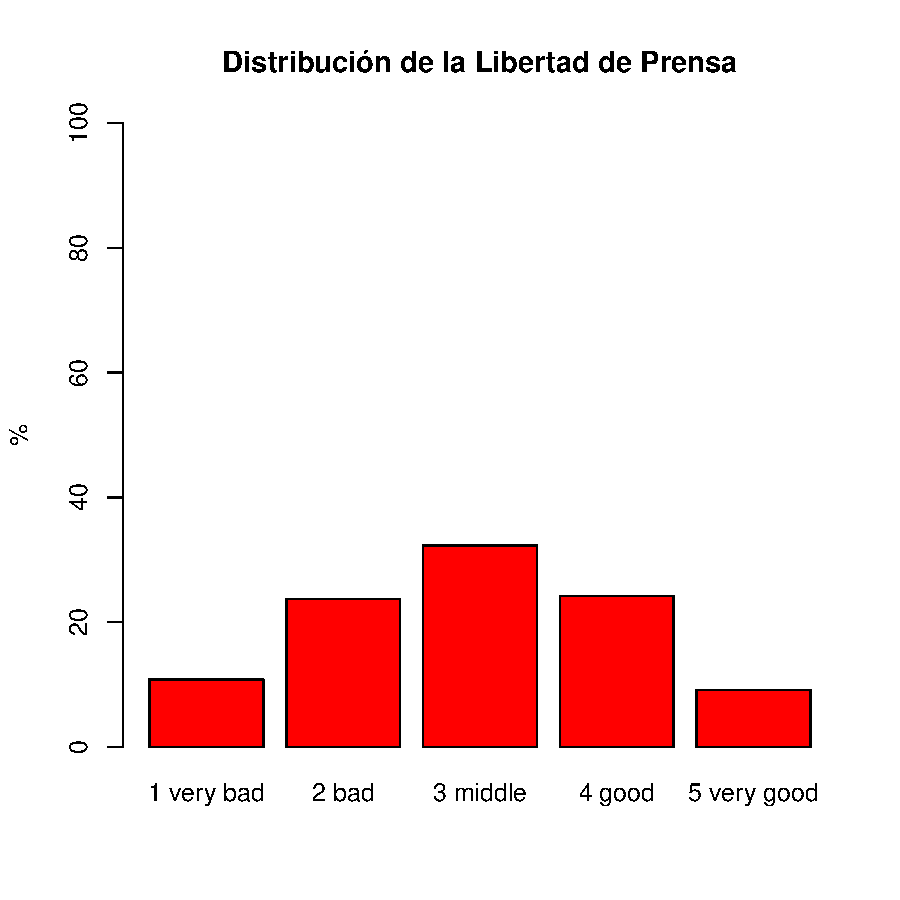
\includegraphics{paperVersion_0-pressTableRelPlot}


Podemos mostrar los estadísticos de cada variable:
\begin{Schunk}
\begin{Sinput}
> summary(dataidx[,-1])
\end{Sinput}
\begin{Soutput}
      gdp         FreedomintheWorld IndexofEconomicFreedom PressFreedomIndex
 Min.   :   700   Min.   :1.000     Min.   :1.000          Min.   :1.000    
 1st Qu.:  4525   1st Qu.:3.000     1st Qu.:2.000          1st Qu.:2.000    
 Median : 13000   Median :3.000     Median :3.000          Median :3.000    
 Mean   : 21667   Mean   :3.409     Mean   :2.661          Mean   :2.973    
 3rd Qu.: 29200   3rd Qu.:5.000     3rd Qu.:3.000          3rd Qu.:4.000    
 Max.   :139100   Max.   :5.000     Max.   :5.000          Max.   :5.000    
 DemocracyIndex       WorldFreedom    EconomicFreedom      PressFreedom
 Min.   :1.000   1 very bad :46    1 very bad :18     1 very bad :20   
 1st Qu.:1.000   3 middle   :56    2 bad      :65     2 bad      :44   
 Median :4.000   5 very good:84    3 middle   :71     3 middle   :60   
 Mean   :2.866                     4 good     :26     4 good     :45   
 3rd Qu.:4.000                     5 very good: 6     5 very good:17   
 Max.   :5.000                                                         
       Democracy 
 1 very bad :50  
 2 bad      :40  
 4 good     :77  
 5 very good:19  
\end{Soutput}
\end{Schunk}


Exploración Bivariada

En este trabajo estamos interesados en el impacto de los otros indices en el nivel de Democracia. Veamos las relaciones bivariadas que tiene esta variable con todas las demás:
\begin{Schunk}
\begin{Sinput}
> explanans=names(dataidx)[c(3:6)]
> corrDem=cor(x=dataidx[,2],
+             y=dataidx[,explanans],
+             use = "na.or.complete",
+             method = "spearman")
> corrDem
\end{Sinput}
\begin{Soutput}
     FreedomintheWorld IndexofEconomicFreedom PressFreedomIndex DemocracyIndex
[1,]         0.3675636               0.655671         0.3510658      0.4804244
\end{Soutput}
\end{Schunk}




Veamos la correlación entre las variables independientes:

\begin{Schunk}
\begin{Sinput}
> corrTable=round(cor(dataidx[explanans],
+                use = "na.or.complete"),2)
> # ocultar media matriz
> corrTable[upper.tri(corrTable)]<-""
> as.data.frame(corrTable)
\end{Sinput}
\begin{Soutput}
                       FreedomintheWorld IndexofEconomicFreedom
FreedomintheWorld                      1                       
IndexofEconomicFreedom              0.48                      1
PressFreedomIndex                   0.83                   0.52
DemocracyIndex                      0.89                   0.58
                       PressFreedomIndex DemocracyIndex
FreedomintheWorld                                      
IndexofEconomicFreedom                                 
PressFreedomIndex                      1               
DemocracyIndex                      0.76              1
\end{Soutput}
\end{Schunk}


Finalmente, vemos los modelos propuestos. Primero sin el índice de democracia como independiente:
\begin{Schunk}
\begin{Sinput}
> LinRegA = lm(gdp ~ ., data = dataidx[,c(2:5)])
> summary(LinRegA)
\end{Sinput}
\begin{Soutput}
Call:
lm(formula = gdp ~ ., data = dataidx[, c(2:5)])

Residuals:
   Min     1Q Median     3Q    Max 
-32063 -11536  -3942   6648 112856 

Coefficients:
                       Estimate Std. Error t value Pr(>|t|)    
(Intercept)              -19595       4707  -4.163 4.85e-05 ***
FreedomintheWorld         -2582       1579  -1.635    0.104    
IndexofEconomicFreedom    14824       1779   8.331 1.89e-14 ***
PressFreedomIndex          3570       2327   1.534    0.127    
---
Signif. codes:  0 ‘***’ 0.001 ‘**’ 0.01 ‘*’ 0.05 ‘.’ 0.1 ‘ ’ 1

Residual standard error: 19420 on 182 degrees of freedom
Multiple R-squared:  0.3554,	Adjusted R-squared:  0.3448 
F-statistic: 33.46 on 3 and 182 DF,  p-value: < 2.2e-16
\end{Soutput}
\begin{Sinput}
> 
\end{Sinput}
\end{Schunk}

Luego incluyendo democracia.

\begin{Schunk}
\begin{Sinput}
> LinRegB = lm(gdp ~ ., data = dataidx[,c(2:6)])
> summary(LinRegB)
\end{Sinput}
\begin{Soutput}
Call:
lm(formula = gdp ~ ., data = dataidx[, c(2:6)])

Residuals:
   Min     1Q Median     3Q    Max 
-28034 -12005  -3782   6375 113275 

Coefficients:
                       Estimate Std. Error t value Pr(>|t|)    
(Intercept)              -18068       4764  -3.793 0.000203 ***
FreedomintheWorld         -5506       2306  -2.388 0.017981 *  
IndexofEconomicFreedom    13575       1911   7.104 2.68e-11 ***
PressFreedomIndex          3571       2314   1.543 0.124564    
DemocracyIndex             4103       2370   1.732 0.085039 .  
---
Signif. codes:  0 ‘***’ 0.001 ‘**’ 0.01 ‘*’ 0.05 ‘.’ 0.1 ‘ ’ 1

Residual standard error: 19320 on 181 degrees of freedom
Multiple R-squared:  0.366,	Adjusted R-squared:  0.3519 
F-statistic: 26.12 on 4 and 181 DF,  p-value: < 2.2e-16
\end{Soutput}
\end{Schunk}





\end{document}
